\section{Constructing a cover} \label{sec:construction-of-cover}
\begin{figure}
    \centering
    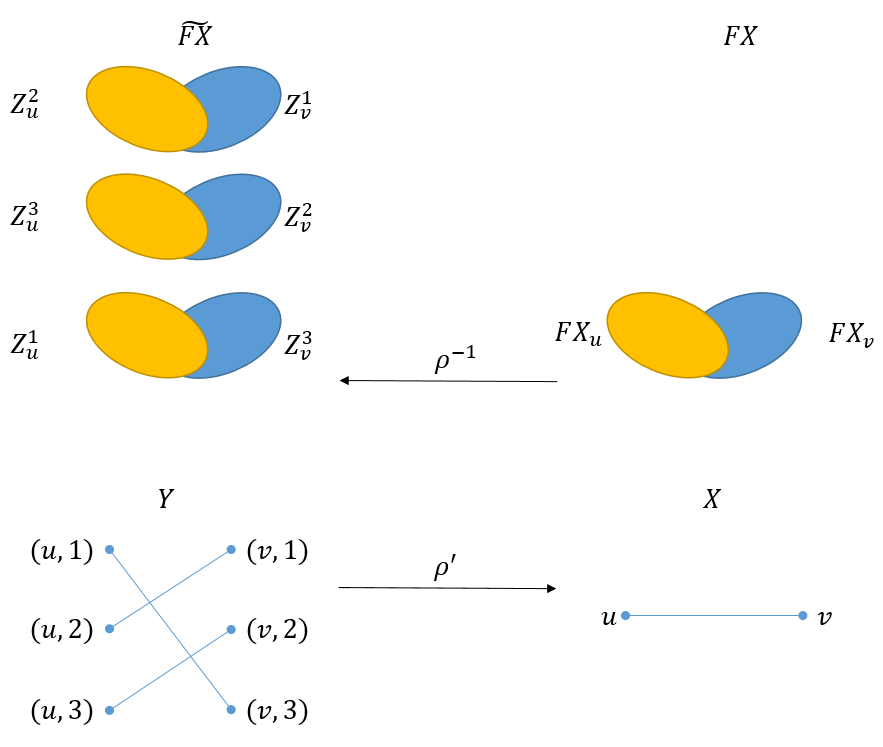
\includegraphics[scale=0.4]{images/cover.png}
    \caption{Constructing a cover of \(X\) from a cover of \(\FX{d_1}X\)}
    \label{fig:cover}
\end{figure}

In this subsection we prove \pref{lem:Y-is-an-honest-to-god-cover-of-X}. We do so in two parts: first we construct a simplicial complex \(Y\) and prove that it covers \(X\). In the second part we explicitly construct the isomorphism \(\iota:\FX{d_1}Y \to \widetilde{\FX{d_1}X}\). In addition to proving \pref{lem:Y-is-an-honest-to-god-cover-of-X}, we will use the explicit definition of \(\iota\) for proving \pref{claim:agreement-with-majority} later on.

Let \(X\) be a \(d\)-dimensional clique complex. Let \(d_1\) be such that \(3d_1 \leq d-2\). Let \(\FX{d_1}X=F(X,d_1)\) be as in \pref{def:face-complex} and assume that \(X\) is well connected as in \pref{def:well-connected-complex}. Fix \(\nu:\widetilde{\FX{d_1}X}\to \FX{d_1}X\) to be an \(\ell\)-cover. In this section, we will show how to construct an $\ell$-cover of \(\rho:Y \to X\) such that \(\widetilde{\FX{d_1}X}\cong \FX{d_1}Y\). 

The main idea will be to encode the vertices \(v \in X(0)\) by the links \(\FX{d_1}X_v \subseteq \FX{d_1}X\) (these are the \(\FX{d_1}X_v = F(X_v,d_1)\) as in \pref{def:face-complex} which are contained as sub complexes inside \(\FX{d_1}X\)). We observe that this encoding has the property that if \(v \sim u\) then \(\FX{d_1}X_v \cap \FX{d_1}X_u = \FX{d_1}X_{uv}\). We will use these non-empty intersections to define the edges in the cover $Y$. For every \(r \in X\), let \(Z_r = \nu^{-1}(\FX{d_1}X_r)\subset \widetilde {\FX{d_1}X}\). Using the well-connectedness of \(X\), we will show that
%
\begin{claim} \label{claim:Z_v-decomposes}~
    \begin{enumerate}
        \item For every non empty \(r \in X^{\leq d_1}\), \(Z_r\) decomposes to exactly \(\ell\) connected-components\footnote{When we say ``connected components'' we mean that the induced complex \(Z_r\) has these \(\ell\) connected components. Of course it may hold that there are paths from \(Z_i\) to \(Z_j\) in \(\widetilde{\FX{d_1}X}\), but they must go through some vertex \(v \in \widetilde{\FX{d_1}X} \setminus Z_r\).} \(Z_r^1,Z_r^2,...,Z_r^\ell \subseteq \widetilde{\FX{d_1}X}\), such that \(\nu\) is an isomorphism between each component and \(\FX{d_1}X_r\), \(\nu|_{Z_r^i}:Z_r^i \overset{\sim}{\to} \FX{d_1}X_r\). 
        \item For every non empty \(r,s \in X^{\leq d_1}\) such that \(r \subseteq s\) there is a permutation \(\pi_{r,s}:[\ell] \to [\ell]\) such that \(Z_{s}^{i} \subseteq Z_{r}^{j}\) if and only if \(\pi_{r,s}(i)=j\).
    \end{enumerate} 
\end{claim}
%
We prove this claim at the end of this subsection. We define the cover \(Y\) of \(X\) as follows. 
Let \(\psi \in C^1(X,Sym(\ell))\) be
\begin{equation} \label{eq:cocycle-def}
    \psi(vu)=\pi_{uv,u}^{-1}\circ \pi_{uv,v}
\end{equation}
where \(\pi_{uv,u},\pi_{uv,v}\) are the permutations promised by the second item of \pref{claim:Z_v-decomposes}. Let \(Y=X^\psi\), i.e. \(Y\) is the clique complex such that \(Y(0)=X \times [\ell]\) and \(\set{(v,i),(u,j)} \in Y(1)\) if \(vu \in X(1)\) and \(j=\psi(vu).i\). Then
\begin{lemma} \label{lem:Y-is-a-cover-of-X}
    \(Y\) is a cover of \(X\). Moreover, it holds that \((v,i) \sim (u,j)\) if and only if \(vu \in X(1)\) and there exists some \(k\) such that \(Z_v^i \cap Z_u^j \supseteq Z_{vu}^k\).
\end{lemma}

For the proof of \pref{lem:Y-is-a-cover-of-X} we use the fact that the \(\pi_{r,s}\) in \pref{claim:Z_v-decomposes} give us a cocycle on the flag complex of \(\FX{d_1}X\) (see below). For this we recall the following corollary: 
\restatecorollary{cor:cocycles-in-flag-complex}
In this notation \(\phi(u,uv)=\pi_{uv,u}\) and thus \(\psi(uv)=\pi_{uv,u}^{-1}\circ \pi_{uv,v}\).


\begin{proof}[Proof of \pref{lem:Y-is-a-cover-of-X}]
    Let us show that \(Y\) is a cover. This is equivalent to showing that \(\psi\) is a cocycle. Let \(X^{\leq 2}\) be the two skeleton of \(X\) and let \(G\) be its flag-complex as in \pref{def:flag-complex}. Let \(\phi:GX(1) \to Sym(\ell)\) be given by \(\phi(r,s)= \pi_{s,r}\) for every \(r \subseteq s\) (where \(\pi_{s,r}\) are the permutations in \pref{claim:Z_v-decomposes}). If we show that \(\phi \in Z^1(GX,Sym(\ell))\) then by \pref{cor:cocycles-in-flag-complex} \(\psi\) is also a cocycle. This amounts to show that for every \(uvw \in X\) it holds that \(\pi_{uvw,uv}\circ \pi_{uv,u} = \pi_{uvw,u}\).

    Indeed, fix \(i\) and let \(k=\pi_{uvw,u}(i)\), and \(k'= \pi_{uvw,uv}\circ \pi_{uv,u}(i)\). By definition this implies that \(Z_{uvw}^k \subseteq Z_u^i\) and that \(Z_{uvw}^{k'} \subseteq Z_{uv}^{\pi_{u,uv}(i)} \subseteq Z_u^i\). The second item of \pref{claim:Z_v-decomposes} says that \(Z_{uvw}^{k'} \subseteq Z_u^i\) implies that  \(k' = \pi_{u,uvw}(i) = k\). 
    
    Next, for the ``moreover'' statement, note that \((v,i) \sim (u,j)\) if and only if there is some \(k\) such that \(\pi_{v,uv}(i)=k\) and such that \(\pi_{u,uv}(j)=k\). This occurs if and only if \(Z_{uv}^k \subset Z_u^i \cap Z_v^j\).
\end{proof}

\begin{proof}[Proof of \pref{claim:Z_v-decomposes}]
Let us start with the first item. We begin by explaining why it is enough to prove it assuming \(r\) is a vertex. Suppose that for every vertex \(v \in X(0)\) it holds that \(Z_v\) decomposes to \(\ell\) connected-components. Let \(r \in X^{\leq d_1}\) and let \(v \in r\) be an arbitrarily chosen vertex inside \(r\). Take \(Z_r^i\) to be the subcomplex induced by \(Z_r^i(0) := Z_v^i(0) \cap \nu^{-1}(\FX{d_1}X_r(0))\). As every \(Z_v^i\) is isomorphic to \(\FX{d_1}X_v\) then in particular, the induced sub-complex \(Z_r^i\) is isomorphic to \(\FX{d_1}X_{r}\). By well connectedness of \(X\), \(\FX{d_1}X_r\) is connected and thus we get that these are \(\ell\) connected-components (they cannot be connected to one another because each lies in a different \(Z_v^i\)).

Now we show the first item for every vertex \(v \in X(0)\). Towards this end, we note that the restriction \(\nu|_{Z_v}:Z_v \to \FX{d_1}X_v\) is also a covering map (for a proof of this statement, see \pref{claim:restriction-of-cover}). From the well connectivity of \(X\), \(\FX{d_1}X_v\) is simply connected, so \(Z_v\) must decompose to \(\ell\) disjoint connected-components. 

We move to the second item. Fix \(r \subseteq s\). We need to show that for every \(i \in [\ell]\) there is a unique \(j\) such that \(Z_s^j \subseteq Z_r^i\), so let us fix some \(i \in [\ell]\). By the first item, the restriction \(\nu|_{Z_r^i}\) is an isomorphism between \(Z_r^i\) and \(\FX{d_1}X_r\). In particular, it follows from the definition of an isomorphism that \(\nu^{-1}(\FX{d_1}X_s) \cap Z_r^i\) is isomorphic (by \(\nu|_{Z_r^i}\)) to \(\FX{d_1}X_s\subset \FX{d_1}X_r\), and thus \(Z_s^j\) is one of the connected components \(Z_s^j \subseteq \nu^{-1}(\FX{d_1}X_s)\) promised by the first item we already proved. This is the index \(j\) we needed. Note that it is unique since \(Z_s^j = \nu^{-1}(\FX{d_1}X_s) \cap Z_r^i\) (so there are no more faces in \(\nu^{-1}(\FX{d_1}X_s)\) and  \(Z_r^i\) that are not already in \(Z_s^j\)).
\end{proof}
%
%

\subsection[The isomorphism between FY to the cover of FX]{The isomorphism between \(\FX{d_1}Y\) to \(\widetilde{\FX{d_1}X}\)}
\begin{figure}
    \centering
    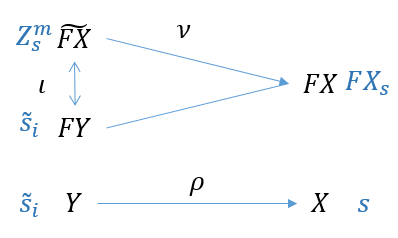
\includegraphics[scale=0.6]{images/commutative-blue.png}
    \caption{Commutative diagram}
    \label{fig:commutative}
\end{figure}
\begin{figure}
    \centering
    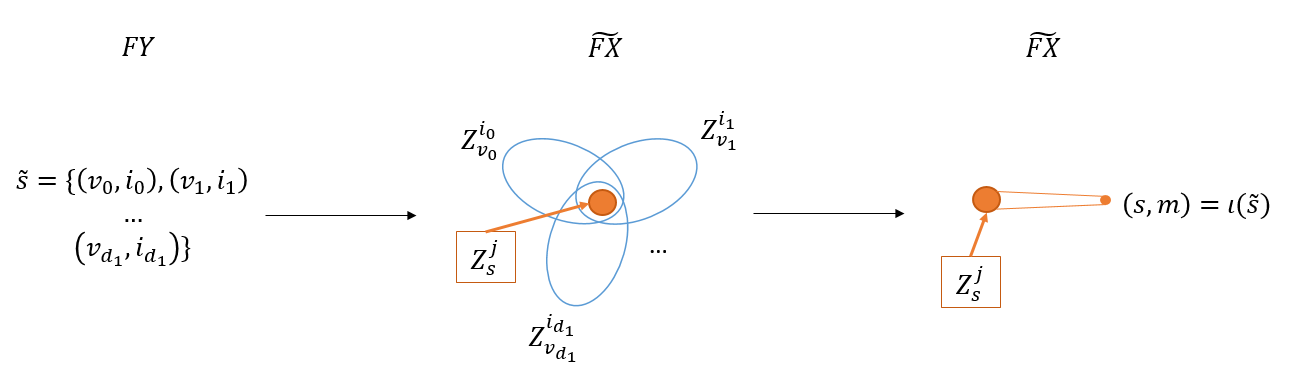
\includegraphics[scale=0.4]{images/iota-description.png}
    \caption{From \(\tilde{s}\) to \(\iota(\tilde{s})=(s,m)\)}
    \label{fig:iota-description}
\end{figure}
%
We continue with the notation in the previous subsection. In this subsection we describe the isomorphism \(\iota:\FX{d_1}Y \to \widetilde{\FX{d_1}X}\) explicitly. See \pref{fig:commutative} for the relations between \(X,Y,\FX{d_1}X,\FX{d_1}Y\) and \(\widetilde{\FX{d_1}X}\).

The idea is simple. Given some \(\tilde{s} = \set{(v_0,i_0),(v_1,i_1),...,(v_{d_1},i_{d_1})} \in \FX{d_1}Y(0)\) , such that \(\rho(\tilde{s})=s = \set{v_0,v_1,\ldots,v_{d_1}}\), 
we need to specify which \(j \in [\ell]\) is such that \(\iota(\tilde{s})=(s,j)\). Using arguments similar to \pref{lem:Y-is-a-cover-of-X}, we will show that the face \(\tilde{s}\) is such that \(\bigcap_{m=0}^{d_1} Z_{v_m}^{i_m}\) contains a ``copy'' \(Z_s^j\) of \(\FX{d_1}X_s\).
%
We will define \(\iota(\tilde{s})=(s,m)\) which is connected to this copy. See \pref{fig:iota-description} for a pictorial description of \(\iota\). We first claim that \(\iota\) is well defined.
\begin{claim} \label{claim:unique-link-of-s}
    Let \(\tilde{s} \in \FX{d_1}Y(0)\),  \(\tilde{s} = \set{(v_0,i_0),(v_1,i_1),...,(v_{d_1},i_{d_1})}\) such that \(\rho(\tilde{s})=s\). Then there is a unique \(j \in [\ell]\) such that \(Z_s^j \subseteq \bigcap_{m=0}^{d_1} Z_{v_m}^{i_m}\).
\end{claim}

We prove this claim below. Assuming it is true, let us show that this is actually an isomorphism.
\begin{lemma}\label{lem:iota-is-an-isomorphism}
    \(\iota:\FX{d_1}Y \to \widetilde{\FX{d_1}X}\) is an isomorphism.
\end{lemma}

\begin{proof}[Proof of \pref{lem:iota-is-an-isomorphism}]
    Let us start by explaining why this is a bijection. First note that for every \(s \in \FX{d_1}X(0)\), \(\iota\) maps the \(\ell\)-elements of \(\rho^{-1}(s) \subseteq \FX{d_1}Y(0)\) to the \(\ell\)-elements of \(\nu^{-1}(s) \subseteq \widetilde{\FX{d_1}X}\). Thus if we show that \(\iota\) is injective, it will also follow that it is a bijection. Let \(\tilde{s}_1, \tilde{s}_2 \in \rho^{-1}(s)\) be distinct elements and we denote \(\iota(\tilde{s}_i)=(s,m_i)\). We'll show that \(m_1 \ne m_2\). Take some vertex \(v \in X(0)\) in \(s \in \FX{d_1}X(0)\), that is \(v \in s=\rho(\tilde{s}_i)\). In particular there are two distinct vertices \((v,i_1),(v,i_2) \in Y(0)\) such that \((v,i_1) \in \tilde{s}_1\) and \((v,i_2) \in \tilde{s}_2\). Note that \(\iota(\tilde{s}_i)\) is the vertex \((s,m_i)\) that is connected to the \(Z_s^{j_i}\) that sits in the intersection \(\bigcap_{(u,k) \in \tilde{s}_i} Z_u^k\). In particular \(Z_s^{j_1} \subseteq Z_v^{i_1}\) and \(Z_s^{j_2} \subseteq Z_v^{i_2}\), thus \(j_1 \ne j_2\), i.e. \((s,m_1)\) and \((s,m_2)\) are connected to different copies of the link of \(s\). In particular this means that \(m_1 \ne m_2\) and the map is injective.
    
    It remains to prove that this is an isomorphism of simplicial complexes. First, we note that both \(\FX{d_1}Y\) and \(\widetilde{\FX{d_1}X}\) are clique complexes:
    \begin{enumerate}
        \item \(X\) is a clique complex, hence by \pref{claim:cover-of-clique-complex} its cover \(Y\) is also a clique complex. The face complex \(\FX{d_1}Y\) of a clique complex is also a clique complex.
        \item \(\FX{d_1}X\) is a clique complex since it is a face complex of a clique complex. By \pref{claim:cover-of-clique-complex} the cover \(\widetilde{\FX{d_1}X}\) is also a clique complex.
    \end{enumerate}
    Thus it is enough to show that the bijection \(\iota\) is a graph isomorphism between \(\FX{d_1}Y^{\leq 1}\) to \((\widetilde{\FX{d_1}X})^{\leq 1}\).
    
    Let us begin by showing that \(\iota\) is a graph homomorphism. Let \(\set{\tilde{s}_1,\tilde{s}_2} \in \FX{d_1}Y(1)\) be an edge. Let \(\iota(\tilde{s}_1) = (s_1,m_1), \iota(\tilde{s}_2)=(s_2,m_2)\). We need to show that \(\set{(s_1,j_1), (s_2,j_2)} \in \widetilde{\FX{d_1}X}(1)\). Since \(\set{\tilde{s}_1,\tilde{s}_2} \in \FX{d_1}Y(1)\), then in particular they are contained in some triangle \(\set{\tilde{s}_1,\tilde{s}_2,\tilde{s}_3} \in \FX{d_1}Y(2)\)\footnote{\(Y\) is pure so \(\FX{d_1}Y\) is also pure.} and denote by \(\nu(\tilde{s}_3)=s_3\). Let \(Z_{s_1}^{j_1}, Z_{s_2}^{j_2}\) be the copies of \(\FX{d_1}X_{s_1},\FX{d_1}X_{s_2}\) such that \((s_1,j_1), (s_2,j_2)\) are connected to \((s_1,m_1),(s_2,m_2)\) respectively (these copies are uniquely determined by the definition of \(\iota\)). If we show that the same copy of \(s_3\) is in the intersection of \(Z_{s_1}^{j_1},Z_{s_1}^{j_2} \subseteq \widetilde{\FX{d_1}X}\), namely that there is some \((s_3,k) \in Z_{s_1}^{j_1} \cap Z_{s_2}^{j_2}\) this will imply that \(\set{(s_1,j_1), (s_2,j_2)} \in \widetilde{\FX{d_1}X}(1)\) (because this implies that both \((s_1,j_1),(s_2,j_2)\) are in the link of \((s_3,k) \in \widetilde{\FX{d_1}X}\). This link is isomorphic by \(\nu\) to the link of \(s_3 \in \FX{d_1}X\). There we know that \(\set{s_1,s_2}\) is an edge, so in particular \(\set{(s_1,j_1), (s_2,j_2)} \in \widetilde{\FX{d_1}X}(1)\)).
    
    Take two vertices \((v_1,k_1),(v_2,k_2) \in Y\) such that \((v_i,k_i) \in \tilde{s}_i\). Because \(\set{\tilde{s}_1,\tilde{s}_2, \tilde{s}_3}  \in \FX{d_1}Y(2)\) implies that \(\tilde{s}_1 \dunion \tilde{s}_2 \dunion \tilde{s}_3 \in Y\). This means that 
    \begin{enumerate}
        \item \(\set{(v_1,k_1),(v_2,k_2)} \in Y(1)\), and that
        \item \(s_3 \in \FX{d_1}X_{v_1 v_2}\).
    \end{enumerate} 
    By \pref{lem:Y-is-a-cover-of-X} the fact that \(\set{(v_1,k_1),(v_2,k_2)} \in Y(1)\) implies that there is a copy \(Z_{v_1,v_2}^{p} \subseteq Z_{v_1}^{k_1} \cap Z_{v_1}^{k_2}\). The fact that \(s_3 \in \FX{d_1}X_{v_1 v_2}\) implies that there is some \((s_3,k) \in Z_{v_1,v_2}^{p}\) and in particular \((s_3,k) \in Z_{v_1}^{k_1},Z_{v_1}^{k_2}\). We now show that this \((s_3,k)\) is the vertex we are looking for. Let \((s_3,k') \in Z_{s_1}^{j_1}\) be the copy of \(s_3\) in \( Z_{s_1}^{j_1}\). by definition of \(\iota\), it holds that \(Z_{s_1}^{j_1} \subseteq Z_{v_1}^{k_1}\). As \(Z_{v_1}^{k_1}\) is isomorphic by \(\nu\) to \(\FX{d_1}X_{v_1}\) and both \((s_3,k),(s_3,k') \in Z_{v_1}^{k_1}\) are sent to \(s_3\) by \(\nu\), this implies that \((s_3,k)=(s_3,k')\). The same argument applies also to \(Z_{s_2}^{j_2}\). We've proven there is an \((s_3,k) \in Z_{s_1}^{k_1} \cap Z_{s_3}^{k_2}\) and this shows that this is a grpah homomorphism.
    
    To be convinced that this is also an isomorphism, note that both \(\widetilde{\FX{d_1}X}\) and \(\FX{d_1}Y\) are $\ell$-covers of \(\FX{d_1}X\). In particular, the degree of every \(\tilde{s} \in \FX{d_1}Y\) is equal to the degree of \(\iota(\tilde{s}) \in \widetilde{\FX{d_1}X}\) (both are equal to the degree of \(\rho(s)\) in \(\FX{d_1}X\)). Any bijective graph isomorphism that preserves degrees must be an isomorphism. 
\end{proof}

\begin{proof}[Proof of \pref{claim:unique-link-of-s}]
    Let \(j\) be such that \(Z_s^j \subseteq Z_{v_0}^{i_0}\) (there is a unique such \(j\) by the second item of \pref{claim:Z_v-decomposes}). We need to show that \(Z_s^j \subseteq Z_{v_m}^{i_m}\) for all \(m=1,2,...,d_1\). Indeed, fix \(m\) and let \(k\) be such that \(Z_{v_0 v_m}^{k} \subseteq Z_{v_0}^{i_0} \cap Z_{v_m}^{i_m}\) (there is such a \(k\) by \pref{lem:Y-is-a-cover-of-X}). Then by the fact that \(\FX{d_1}X_{s} \subseteq \FX{d_1}X_{v_0 v_m} \subseteq \FX{d_1}X_{v_0}\) and \(\FX{d_1}X_{s} \subseteq \FX{d_1}X_{v_0 v_m} \subseteq \FX{d_1}X_{v_m}\), it holds by the isomorphism that \(\nu\) induces that \(Z_s^j \subseteq Z_{v_0 v_m}^k \subseteq Z_{v_0}^{i_0}\), and that \(Z_s^j \subseteq Z_{v_0 v_m}^k \subseteq Z_{v_m}^{i_m}\). In particular \(Z_s^j \subseteq Z_{v_m}^{i_m}\). This shows existence of \(Z_s^j\). For uniqueness we note that there is a unique \(j\) such that \(Z_s^j \subseteq Z_{v_0}^{i_0}\), and \(\bigcap_{m=0}^{d_1} Z_{v_m}^{i_m} \subseteq Z_{v_0}^{i_0}\) so there must be only a single such \(j\).
\end{proof}